 \section{OpenGL}
\label{sec:opengl}

In diesem Abschnitt wird das OpenGL-Framework vorgestellt, das in der
Implementierung verwendet wurde. Es wird nur ein grober Überblick
gegeben und speziell auf die programmierbaren Shader eingegangen, da
diese im Weiteren noch von größerer Bedeutung sind. Es werden bei der
Erklärung teilweise OpenCL-Begriffe verwendet, da sich gewisse
Unterschiede und Gemeinsamkeiten zwischen den Frameworks ergeben.

OpenGL stellt eine Programmierschnittstelle bereit, welche abstrakte
Operationen zum Darstellen von Grafik mit der GPU zur Verfügung
stellt. Der Aufbau der Komponenten, die zum Rendering nötig sind, wird
in dem Modell der Grafik- bzw. Rendering-Pipeline zusammengefasst
(siehe \cref{fig:opengl_graphics_pipeline}).

\begin{figure}[ht]
\centering
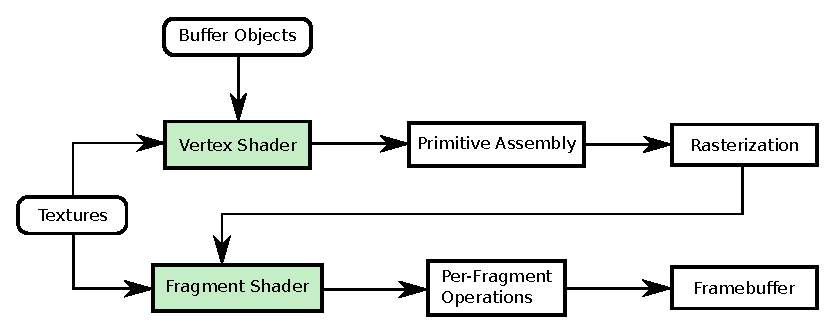
\includegraphics[width=15cm]{images/graphics_pipeline}
\caption{Die OpenGL-Grafikpipeline. Programmierbare Schnittstellen sind hervorgehoben.}
\label{fig:opengl_graphics_pipeline}
\end{figure}

Wie in OpenCL gibt es grundsätzlich zwei Datenstrukturen, die in
OpenGL als Eingabe fungieren können: Buffer und Texturen. Buffer
werden im Allgemeinen zur Speicherung geometrischer Daten verwendet,
\Pimiddydh{} Arrays von Vertizes und Primitiven. Texturen gleichen image
objects in OpenCL\@. Es sind mehrdimensionale Datenstrukturen mit
speziell definierten Attributen und Operationen, die \PimiddyzB{}
verschiedene Arten von Interpolation erlauben. Sie können ein-, zwei-
oder dreidimensionale Bilddaten repräsentieren.

Die zu verarbeitenden Objekte liegen als Vertizes in einer definierten
Reihenfolge in Form von Vertex- und Indexbuffern vor. Beim Zeichnen
gibt man eine Topologie für diese Vertizes an. In dieser Arbeit werden
Punkte (Point Sprites) und Dreiecke als Topologien
verwendet. Dreiecksnetze nennt man auch \PimiddyBegriff{Meshes}. Sie
werden \PimiddyzB{} aus einer Modeldatei geladen oder algorithmisch
erstellt (siehe \cref{sec:fallen_snow}).

Die einzelnen Vertizes werden über einen \PimiddyBegriff{Vertex Shader}
verarbeitet, der als Ausgabe Vertexattribute setzt oder modifiziert,
wie etwa Position, Texturkoordinaten und Normalen. Die transformierten
Vertizes werden dann über fest eingebaute, \Pimiddydh{} nicht
programmierbare, Verarbeitungsschritte zu Grafikprimitiven
zusammengesetzt und gerastert.

Dabei wird bestimmt, welche Teile der Geometrie sichtbar sind und
welche Primitive welche Bereiche des Bildes (\PimiddyzB{} Framebuffer)
überdecken. Das Ergebnis der Rasterung sind Fragments, die im
\PimiddyBegriff{Fragment Shader} manipuliert werden können. Ein
Fragment ist eine Datenstruktur, welche die zu einem einzelnen Pixel
gehörigen Daten eines Primitivs enthält. Mehrere Fragments können zu
einem Pixel gehören, etwa bei überlappender Geometrie, aber ein
Fragment beeinflusst immer nur höchstens ein Pixel des fertigen
Bildes.

Jedes Fragment besteht aus festen Datenfeldern, wie Tiefeninformation
und Bildschirmkoordinaten. Zusätzlich kann das Shaderprogramm
beliebige weitere vertexbezogene Daten vom Vertexshader übergeben
bekommen. Die Transformierung von Vertexdaten in Fragmentdaten
geschieht im Rasterungsschritt durch Interpolation. Die Ausgabe eines
Fragmentshaders besteht aus Farb- und Tiefeninformation, die am Ende
der Pipeline in eine spezielle Datenstruktur, den sogenannten
Framebuffer, geschrieben werden. Im einfachsten Fall ist dies der
Puffer, der das am Bildschirm dargestellte Bild im Speicher der
Grafikkarte repräsentiert. Es sind aber über sogenannte Framebuffer
Objects auch andere benutzerdefinierte Ausgaben möglich, die
geschrieben und \PimiddyzB{} als Texturen in weiteren Renderdurchgängen
durch die Pipeline wiederum als Input für andere Shader verwendet
werden können.  Die in dieser Arbeit verwendeten Shader sind in der
OpenGL Shading Language (GLSL) geschrieben, einer höheren
Programmiersprache mit C-ähnlicher Syntax, die zur Ausführung auf der
Grafikkarte mit OpenGL zu binärem Shadercode kompiliert wird.

Alle Versionen von GLSL unterstützen if-else-Verzweigungskonstrukte
wie in C und Schleifen.  Hardware mit voller Unterstützung für OpenGL
2.0, mit der Einführung von GLSL, wurde um 2003--2004 sowohl von NVidia
als auch von ATI auf den Markt gebracht.
